\FILENAME

\section*{Basic Statistics with Hadoop}       

The idea of this exercise is to get you started with Hadoop and the
MapReduce concept. You may have already looked at the WordCount
example, both serial and Hadoop implementations. This problem is
similar to WordCount except that you will be computing the basic
statistics such as min, max, average, and standard deviation of a
given data set.

The input to the program will be a text file carrying exactly one
floating point number per line. The output should include {\em min,
  max, average, and standard deviation} f these numbers.

\begin{figure}[!htbp]
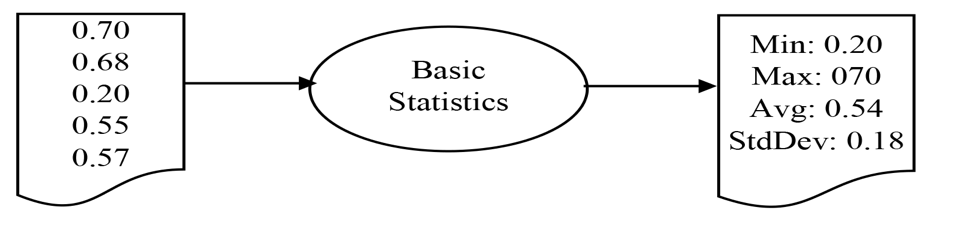
\includegraphics[width=8cm,height=3cm]{section/icloud/assignment/problems/project1/p1example.png}
\centering
\end{figure}

\subsection*{Files}

A test input file is available as a separate attachment.  The
statistics values for this input are {\em Min: 0.01 Max: 0.99 Avg:
  0.50 StdDev: 0.2817}

\slides{Assignments}{Project 1}{Input Data}{https://drive.google.com/open?id=0B88HKpainTSfcUlZX3BpV05TRDg}

\subsection*{Deliverables}

You will need to complete the source code and write a report. Zip your
work into a file with the name \verb|username_exercise1.zip| (replace
{\em username} with your own) and submit the following:

\begin{itemize}
\item Complete source code
\item A document with the following details:

  \begin{itemize}
  \item	Transformation of data during the computations, i.e. data type of key, value
  \item	The data structure used to transfer between Map and Reduce phases
  \item	How the data flow happens through disk and memory during the computation
  \end{itemize}

\end{itemize}

\subsection*{Evaluation}

The point total for this exercise is 5.

\begin{itemize}
\item Correctness of the source code (2 points)
\item	Completeness of the report (3 points)
\end{itemize}

